% --------------------------------------------------------------------------
%   main.tex © 2026 J. G. Silva | lavradodosilicio@gmail.com
% --------------------------------------------------------------------------
%   Última modificação: 12/11/2026
% --------------------------------------------------------------------------
\documentclass[aspectratio=169,10pt]{beamer}

\usepackage[utf8]{inputenc}
\usepackage[T1]{fontenc}
\usepackage[brazilian]{babel}
\usepackage{helvet}
\renewcommand{\familydefault}{\sfdefault}
\usepackage{amsmath,amssymb}
\usepackage{booktabs,array,multirow}
\usepackage{tikz,pgfplots}
\pgfplotsset{compat=1.16}
\usetikzlibrary{calc,arrows.meta,positioning}
\usepackage{listings}

% Informações gerais
\newcommand{\autor}{Janderson Gomes}
\newcommand{\disciplina}{Estrutura de Dados}
\newcommand{\professor}{Prof. Dr. Filipe Dwan Pereira}
\newcommand{\programa}{Programa de Pós Graduação em Computação Aplicada - PPCA}
\newcommand{\linha}{Mestrado Profissional em Informática na Educação}
\newcommand{\instituicao}{Universidade Federal de Roraima - UFRR}
\newcommand{\datapres}{Novembro de 2026}

% Paleta de cores (Mondrian)
\definecolor{mred}{RGB}{200,52,45}
\definecolor{mblue}{RGB}{36,82,158}
\definecolor{myel}{RGB}{242,201,76}
\definecolor{mgold}{RGB}{206,160,24}
\definecolor{mink}{RGB}{28,28,28}
\definecolor{mpaper}{RGB}{252,251,247}
\definecolor{mgrey}{RGB}{120,120,115}
\colorlet{seccol}{mred}
\colorlet{seccolb}{myel}
\newcommand{\setsec}[2]{\colorlet{seccol}{#1}\colorlet{seccolb}{#2}}

% Tema
\setbeamertemplate{navigation symbols}{}
\setbeamercolor{normal text}{fg=mink,bg=mpaper}
\setbeamercolor{structure}{fg=mink}
\setbeamercolor{block title}{fg=white,bg=mblue}
\setbeamercolor{block body}{fg=mink,bg=mpaper}
\setbeamercolor{block title alerted}{fg=white,bg=mred}
\setbeamercolor{block body alerted}{fg=mink,bg=mpaper}
\setbeamercolor{block title example}{fg=mink,bg=myel}
\setbeamercolor{block body example}{fg=mink,bg=mpaper}
\setbeamerfont{block title}{size=\footnotesize,series=\bfseries}
\setbeamersize{text margin left=1.1cm,text margin right=1.9cm}
\setbeamertemplate{itemize item}{\raisebox{0.15ex}{\textcolor{seccol}{\rule{0.55ex}{0.55ex}}}}
\setbeamertemplate{itemize subitem}{\raisebox{0.15ex}{\textcolor{mink}{\rule{0.4ex}{0.4ex}}}}
\setbeamertemplate{enumerate item}{\insertenumlabel.}
\setbeamercolor{enumerate item}{fg=mink}
\setbeamertemplate{bibliography item}[text]
\setbeamercolor{bibliography item}{fg=mink}
\setbeamerfont{bibliography item}{size=\tiny}
\setbeamerfont{bibliography entry author}{size=\tiny}
\setbeamerfont{bibliography entry title}{size=\tiny}
\setbeamerfont{bibliography entry location}{size=\tiny}
\setbeamerfont{bibliography entry note}{size=\tiny}

\setbeamertemplate{background canvas}{%
 \begin{tikzpicture}[remember picture,overlay]
  \fill[mpaper] (current page.south west) rectangle (current page.north east);
  % faixa lateral: linhas pretas e dois blocos de cor (nunca se tocam)
  \fill[mink] ($(current page.north east)+(-1.45,0)$) rectangle ($(current page.south east)+(-1.35,0)$);
  \fill[seccol] ($(current page.north east)+(-1.35,0)$) rectangle ($(current page.north east)+(0,-1.55)$);
  \fill[mink] ($(current page.north east)+(-1.35,-1.55)$) rectangle ($(current page.north east)+(0,-1.65)$);
  \fill[mink] ($(current page.south east)+(-1.35,1.25)$) rectangle ($(current page.south east)+(0,1.35)$);
  \fill[seccolb] ($(current page.south east)+(-1.35,0)$) rectangle ($(current page.south east)+(0,1.25)$);
 \end{tikzpicture}}

\setbeamertemplate{frametitle}{%
 \vspace{0.6em}%
 \noindent\raisebox{-0.1ex}{\textcolor{seccol}{\rule{0.9ex}{0.9ex}}}\hspace{0.6em}%
 {\Large\bfseries\color{mink}\insertframetitle\par}%
 \vspace{-0.2em}\noindent{\color{mink}\rule{\linewidth}{1.3pt}}\par\vspace{0.2em}}

\setbeamertemplate{footline}{%
 \leavevmode\hbox to \paperwidth{\hspace*{1.1cm}%
 {\fontsize{6}{7}\selectfont\color{mgrey}\autor \,·\, Quick Sort \,·\, \disciplina\ \,·\, UFRR}%
 \hfill{\fontsize{7}{8}\selectfont\color{mink}\insertframenumber\,/\,\inserttotalframenumber}\hspace*{1.8cm}}%
 \vskip0.3cm}

% Códigos
\lstdefinelanguage{plain}{}
\lstdefinestyle{code}{
  language=C, basicstyle=\ttfamily\fontsize{7}{8.5}\selectfont\color{mink},
  keywordstyle=\bfseries\color{mblue}, commentstyle=\itshape\color{mgrey},
  numbers=left, numberstyle=\tiny\color{mgrey}, numbersep=5pt,
  frame=l, rulecolor=\color{mink}, framerule=1.2pt, xleftmargin=11pt,
  showstringspaces=false, columns=fullflexible, keepspaces=true,
  literate={á}{{\'a}}1 {à}{{\`a}}1 {ã}{{\~a}}1 {â}{{\^a}}1 {é}{{\'e}}1
    {ê}{{\^e}}1 {í}{{\'i}}1 {ó}{{\'o}}1 {ô}{{\^o}}1 {õ}{{\~o}}1 {ú}{{\'u}}1
    {ç}{{\c c}}1 {Á}{{\'A}}1 {É}{{\'E}}1 {Ç}{{\c C}}1
    {←}{{$\leftarrow$}}1 {↔}{{$\leftrightarrow$}}1 {≤}{{$\leq$}}1
    {≥}{{$\geq$}}1 {−}{{-}}1 {▷}{{$\triangleright$}}1}
\lstdefinestyle{pseudo}{style=code, language=plain,
  basicstyle=\fontsize{7.6}{9.3}\selectfont\color{mink}, escapechar=|}
\lstdefinestyle{codesmall}{style=code, basicstyle=\ttfamily\fontsize{6.4}{7.8}\selectfont\color{mink}}
\newcommand{\kw}[1]{\textbf{#1}}
\newcommand{\tagbox}[3]{\colorbox{#1}{\textcolor{#2}{\strut\scriptsize\bfseries\ #3\ }}}
\newcommand{\pv}[1]{\colorbox{mred}{\textcolor{white}{\strut\bfseries #1}}}

% Figuras
\newcommand{\figbox}[4]{% arquivo, largura, altura, texto-guia
 \IfFileExists{#1}{\includegraphics[width=#2,height=#3,keepaspectratio]{#1}}{%
 \begin{tikzpicture}
  \draw[mink,dashed,line width=0.7pt] (0,0) rectangle (#2,#3);
  \node[text width=\dimexpr#2-0.6cm\relax,align=center,font=\scriptsize,text=mgrey]
   at ({\dimexpr#2/2\relax},{\dimexpr#3/2\relax}) {#4};
 \end{tikzpicture}}}

% Arrays ou vetores
% \qarr{lista}{i}{s}{p}: Lomuto. vermelho=pivô, azul=região < pivô,
% amarelo=elemento examinado (i). Marcadores: i (acima), s (abaixo).
\newcommand{\qarr}[4]{%
 \begin{tikzpicture}[baseline=(b.base)]
  \node (b) at (0,0) {\strut};
  \foreach \v [count=\k from 0] in {#1}{%
    \def\cf{mpaper}\def\ct{mink}%
    \ifnum\k<#3 \def\cf{mblue}\def\ct{white}\fi
    \ifnum\k=#2 \def\cf{myel}\def\ct{mink}\fi
    \ifnum\k=#4 \def\cf{mred}\def\ct{white}\fi
    \node[draw=mink,line width=0.8pt,fill=\cf,minimum size=0.7cm,inner sep=0pt,
          text=\ct,font=\bfseries] at (\k*0.86,0) {\v};}%
  \ifnum#2<7 \node[font=\scriptsize\itshape] at (#2*0.86,0.58) {$i$};\fi
  \ifnum#3<7 \node[font=\scriptsize\itshape] at (#3*0.86,-0.58) {$s$};\fi
 \end{tikzpicture}}
% \carr{v/cor/texto,...}: cores explícitas
\newcommand{\carr}[1]{%
 \begin{tikzpicture}[baseline=(b.base)]
  \node (b) at (0,0) {\strut};
  \foreach \v/\c/\t [count=\k from 0] in {#1}{%
    \node[draw=mink,line width=0.8pt,fill=\c,minimum size=0.7cm,inner sep=0pt,
          text=\t,font=\bfseries] at (\k*0.86,0) {\v};}%
 \end{tikzpicture}}
% \tarr{lista}{lt}{i}{gt}: três vias. azul <p, amarelo =p, vermelho >p
\newcommand{\tarr}[4]{%
 \begin{tikzpicture}[baseline=(b.base)]
  \node (b) at (0,0) {\strut};
  \foreach \v [count=\k from 0] in {#1}{%
    \def\cf{mpaper}\def\ct{mink}%
    \ifnum\k<#3 \def\cf{myel}\def\ct{mink}\fi
    \ifnum\k<#2 \def\cf{mblue}\def\ct{white}\fi
    \ifnum\k>#4 \def\cf{mred}\def\ct{white}\fi
    \node[draw=mink,line width=0.8pt,fill=\cf,minimum size=0.7cm,inner sep=0pt,
          text=\ct,font=\bfseries] at (\k*0.86,0) {\v};}%
  \node[font=\scriptsize\itshape] at (#3*0.86,0.58) {$i$};
  \node[font=\scriptsize\itshape] at (#2*0.86,-0.58) {$lt$};
  \node[font=\scriptsize\itshape] at (#4*0.86,-0.58) {$gt$};
 \end{tikzpicture}}

% Gráficos
\pgfplotsset{mond/.style={axis lines=left, axis line style={mink,line width=1pt},
  tick style={mink}, tick label style={font=\tiny}, label style={font=\scriptsize},
  title style={font=\scriptsize\bfseries}, legend style={font=\tiny,draw=none,fill=none},
  every axis plot/.append style={line width=1pt}}}

\newcommand{\nb}[3]{\tikz[baseline=-0.6ex]\node[fill=#1,text=#2,minimum size=0.55cm,inner sep=0pt,font=\bfseries\small]{#3};}
\newcommand{\ev}[5]{% x, pos(1 acima/-1 abaixo), cor, ano, texto
 \fill[#3] (#1-0.17,-0.17) rectangle (#1+0.17,0.17);
 \draw[mink,line width=0.6pt] (#1,#2*0.17) -- (#1,#2*0.62);
 \ifnum#2>0 \node[anchor=south,text width=2.4cm,align=center,font=\tiny] at (#1,0.65) {\textbf{#4}\\#5};
 \else \node[anchor=north,text width=2.4cm,align=center,font=\tiny] at (#1,-0.65) {\textbf{#4}\\#5};\fi}

 \newcommand{\chip}[1]{\tikz[baseline=0.05ex]\draw[mink,line width=0.6pt,fill=#1] (0,0) rectangle (0.27,0.27);}

% Abertura de seção
\newcommand{\secslide}[6]{% num, título, c1, c2, c3, cor do número
 \begin{frame}[plain]
  \begin{tikzpicture}[remember picture,overlay]
   \begin{scope}[shift={(current page.south west)}]
    \fill[mpaper] (0,0) rectangle (16,9);
    \fill[#3] (0,6.34) rectangle (3.0,9);
    \fill[#4] (12.74,0) rectangle (16,1.46);
    \fill[#5] (12.74,6.34) rectangle (16,9);
    \fill[mink] (3.0,0) rectangle (3.14,9);
    \fill[mink] (12.6,0) rectangle (12.74,9);
    \fill[mink] (0,6.2) rectangle (16,6.34);
    \fill[mink] (3.14,1.46) rectangle (16,1.6);
    \node[text=#6,font=\fontsize{44}{44}\bfseries] at (1.5,7.7) {#1};
    \node[anchor=west,text width=8.6cm,align=left,font=\fontsize{24}{28}\bfseries,text=mink] at (3.6,3.6) {#2};
   \end{scope}
  \end{tikzpicture}
 \end{frame}}

\title{Quick Sort}
\begin{document}

% Capa
\begin{frame}[plain]
 \begin{tikzpicture}[remember picture,overlay]
  \begin{scope}[shift={(current page.south west)}]
   \fill[mpaper] (0,0) rectangle (16,9);
   \fill[mred]  (0,6.64) rectangle (3.0,9);
   \fill[myel]  (13.14,6.64) rectangle (16,9);
   \fill[mblue] (13.14,0) rectangle (16,1.86);
   \fill[mink] (3.0,0) rectangle (3.14,9);
   \fill[mink] (13.0,0) rectangle (13.14,9);
   \fill[mink] (0,6.5) rectangle (16,6.64);
   \fill[mink] (3.14,1.72) rectangle (16,1.86);
   \fill[mink] (0,4.3) rectangle (3.0,4.44);
   \node[anchor=west,font=\scriptsize\bfseries,text=mgrey,text width=9.5cm] at (3.5,7.9)
     {\MakeUppercase{\instituicao}\\[2pt]\MakeUppercase{\programa\\\linha}};
   \node[anchor=west,font=\fontsize{46}{50}\bfseries,text=mink] at (3.5,5.2) {Quick Sort};
   %\node[anchor=west,font=\large,text=mink,text width=9.2cm] at (3.5,3.75)
     %{Ordenação por particionamento: do algoritmo de Hoare às variantes modernas};
   \node[anchor=west,font=\small,text=mink,text width=9.2cm] at (3.5,2.45)
     {\textbf{\autor}}; 
   \node[anchor=west,font=\small,text=mink,text width=9.2cm] at (3.5,0.75)
     {\textbf{\disciplina} | \professor\\ \datapres};
  \end{scope}
 \end{tikzpicture}
\end{frame}

% Menu da parada
\begin{frame}{Conteúdo}
 \begin{columns}[T]
  \column{0.49\textwidth}
   \vspace{0.4em}
   \nb{mred}{white}{1}\ \ Contexto histórico\\[1.1ex]
   \nb{mblue}{white}{2}\ \ O algoritmo\\[1.1ex]
   \nb{myel}{mink}{3}\ \ Passo a passo com 6 números\\[1.1ex]
   \nb{mred}{white}{4}\ \ Variações e versões modernas
  \column{0.49\textwidth}
   \vspace{0.4em}
   \nb{mblue}{white}{5}\ \ Análise de complexidade\\[1.1ex]
   \nb{myel}{mink}{6}\ \ Resultados experimentais\\[1.1ex]
   \nb{mred}{white}{7}\ \ Comparações\\[1.1ex]
   \nb{mblue}{white}{8}\ \ Usos, vantagens, limitações
 \end{columns}
 \vfill
 %\begin{block}{Legenda nas figuras}
 % \footnotesize\carr{p/mred/white,<p/mblue/white,i/myel/mink,\ldots/mpaper/mink}\hspace{0.8em}
 % vermelho = pivô \ · \ azul = menores que o pivô \ · \ amarelo = elemento em exame
 %\end{block}
 %\begin{block}{Legenda nas figuras}
  %\footnotesize\carr{p/mred/white,<p/mblue/white,i/myel/mink,\ldots/mpaper/mink}\hspace{0.8em}
  %pivô \ · \ menores que o pivô \ · \ elemento em exame \ · \ geral.  
 %\end{block}
 %\vspace{0.5em}
\end{frame}

% Contexto histórico
\setsec{mred}{myel}
\secslide{1}{Contexto histórico}{mred}{mblue}{myel}{white}

\begin{frame}{O problema da ordenação}
 \begin{columns}[T]
  \column{0.56\textwidth}
   \small Dada uma sequência de $n$ registros $\langle a_1,a_2,\dots,a_n\rangle$, ordenar é encontrar uma permutação
   $\langle a'_1,a'_2,\dots,a'_n\rangle$ tal que
   \[ a'_1\le a'_2\le\cdots\le a'_n \]
   para uma relação de ordem sobre as chaves \cite{knuth98,clrs22}.
   \vspace{0.3em}
   \footnotesize
   \begin{itemize}
    \item \textbf{Por quê?} Ordenar acelera a busca (busca binária, $O(\log n)$), a detecção de duplicatas e a intercalação de conjuntos.
    \item \textbf{Modelo de custo:} comparações entre chaves e movimentações de registros \cite{knuth98}.
    \item \textbf{Limite inferior:} qualquer ordenação por comparações exige $\Omega(n\log n)$ comparações no pior caso \cite{clrs22}.
   \end{itemize}
  \column{0.3035\textwidth}
   \begin{exampleblock}{Propriedades que usaremos}
    \footnotesize
    \textbf{In-place:} usa $O(1)$ ou $O(\log n)$ de memória extra.\\[0.3ex]
    \textbf{Estável:} preserva a ordem relativa de chaves iguais.\\[0.3ex]
    \textbf{Adaptativo:} aproveita ordem parcial já existente.
   \end{exampleblock}
 \end{columns}
\end{frame}

\begin{frame}{Tony Hoare e a invenção do Quick Sort}
 \begin{columns}[T]
  \column{0.30\textwidth}
   \centering
   \figbox{img/hoare.png}{3.6cm}{4.6cm}{Foto de C.~A.~R.~Hoare\\(ex.: Wikimedia Commons, observar a licença)\\arquivo \texttt{img/hoare.jpg}}
  \column{0.55\textwidth}
   \footnotesize
   \begin{itemize}
    \item \textbf{C. A. R. (Tony) Hoare} (n.\ 1934), cientista da computação britânico; Prêmio Turing de 1980 por contribuições ao projeto e à definição de linguagens de programação.
    \item \textbf{1959--60:} estudante visitante na Universidade Estatal de Moscou, trabalhando com tradução automática; precisou ordenar palavras para consulta a um dicionário e concebeu o Quick Sort \cite{shustek09}.
    \item \textbf{1961:} publicado como \emph{Algorithm 64: Quicksort} (\emph{Communications of the ACM}) \cite{hoare61}; \textbf{1962:} artigo completo com análise, no \emph{The Computer Journal} \cite{hoare62}.
    \item Na mesma época, \emph{Algorithm 65: Find} (hoje \emph{quickselect}) usa a mesma partição para achar o $k$-ésimo menor elemento \cite{hoare61find}.
   \end{itemize}
 \end{columns}
\end{frame}

\begin{frame}{Linha do tempo}
 \centering
 \begin{tikzpicture}[x=1cm,y=1cm]
  \draw[mink,line width=1.6pt] (0,0) -- (12.9,0);
  \ev{1.25}{1}{mred}{1959--61}{Hoare concebe e publica o Quick Sort (Algorithm 64)}
  \ev{2.55}{-1}{mblue}{1962}{Artigo \emph{Quicksort}, The Computer Journal}
  \ev{3.85}{1}{myel}{1976}{Dijkstra: bandeira holandesa (base das três vias)}
  \ev{5.15}{-1}{mred}{1978}{Sedgewick: análise e otimizações (mediana de 3, corte)}
  \ev{6.45}{1}{mblue}{1993}{Bentley \& McIlroy: \emph{sort} de biblioteca (3 vias, ninther)}
  \ev{7.75}{-1}{myel}{1997}{Musser: Introsort, pior caso $O(n\log n)$}
  \ev{9.05}{1}{mred}{2009}{Yaroslavskiy: Dual-Pivot (adotado no Java 7)}
  \ev{10.35}{-1}{mblue}{2016}{BlockQuicksort (Edelkamp \& Weiss)}
  \ev{11.65}{1}{myel}{2021}{pdqsort (Peters), usado no Go 1.19}
 \end{tikzpicture}
 \par\vspace{0.8em}
 {\scriptsize Fontes: \cite{hoare61,hoare62,dijkstra76,sedgewick78,bentleymcilroy93,musser97,wildnebel12,edelkampweiss16,peters21}.}
\end{frame}

% O Algoritmo
\setsec{mblue}{mred}
\secslide{2}{O algoritmo}{mblue}{myel}{mred}{white}

\begin{frame}{Ideia central: dividir e conquistar}
 \begin{columns}[T]
  \column{0.46\textwidth}
   \begin{enumerate}
    \item \textbf{Escolher} um elemento, o \emph{pivô}.
    \item \textbf{Particionar} o vetor: elementos menores que o pivô à esquerda, os demais à direita; o pivô fica em sua posição definitiva.
    \item \textbf{Recursão} nas duas partes.
   \end{enumerate}
   \vspace{0.6em}
   Não há etapa de ``combinação'': ao final das chamadas, o vetor já está ordenado \cite{clrs22}.
  \column{0.60\textwidth}
   \centering\vspace{0.6em}
   \begin{tikzpicture}
    \draw[mink,line width=0.8pt,fill=mblue] (0,0) rectangle (2.3,0.9);
    \node[text=white,font=\small\bfseries] at (1.15,0.45) {$< p$};
    \draw[mink,line width=0.8pt,fill=mred] (2.6,0) rectangle (3.4,0.9);
    \node[text=white,font=\small\bfseries] at (3.0,0.45) {$p$};
    \draw[mink,line width=0.8pt,fill=mpaper] (3.7,0) rectangle (6.0,0.9);
    \node[font=\small\bfseries] at (4.85,0.45) {$\ge p$};
    \draw[mink,line width=0.8pt,-{Stealth}] (1.15,-0.15) -- (1.15,-0.75) node[below,font=\scriptsize] {$\underbrace{A[lo..q-1]}_{\textrm{menores}}\quad$};
    \draw[mink,line width=0.8pt,-{Stealth}] (3.0,-0.15) -- (3.0,-0.75)
    node[below,font=\scriptsize] {$\underbrace{A[q]}_{\textrm{pivô}}$};
    \draw[mink,line width=0.8pt,-{Stealth}] (4.85,-0.15) -- (4.85,-0.75) node[below,font=\scriptsize] {$\underbrace{A[q+1..hi-1]}_{\textrm{maiores}}$};
   \end{tikzpicture}
   \vspace{0.3em}\par
   {\footnotesize Vetor após a partição.}
 \end{columns}
\end{frame}

\begin{frame}[fragile]{QuickSort: pseudocódigo e C}
 \begin{columns}[T]
  \column{0.44\textwidth}
   \tagbox{mblue}{white}{Pseudocódigo}\vspace{0.3em}
\begin{lstlisting}[style=pseudo]
QUICKSORT(A, lo, hi)
1  |\kw{se}| lo < hi |\kw{então}|
2      p ← PARTICIONAR(A, lo, hi)
3      QUICKSORT(A, lo, p − 1)
4      QUICKSORT(A, p + 1, hi)
\end{lstlisting}
   \vspace{0.5em}
   \begin{alertblock}{Primeira chamada}
    \footnotesize\texttt{QUICKSORT(A, 0, n - 1)}, com índices inclusivos e base 0.
   \end{alertblock}
  \column{0.54\textwidth}
   \tagbox{mred}{white}{Linguagem C}\vspace{0.3em}
\begin{lstlisting}[style=code]
void quicksort(int A[], int lo, int hi) {
    if (lo < hi) {
        int p = particionar(A, lo, hi);
        quicksort(A, lo, p - 1);
        quicksort(A, p + 1, hi);
    }
}
\end{lstlisting}
 \end{columns}
\end{frame}

\begin{frame}[fragile]{Partição de Lomuto (pivô = último elemento)}
 \begin{columns}[T]
  \column{0.46\textwidth}
   \tagbox{mblue}{white}{Pseudocódigo}\vspace{0.3em}
\begin{lstlisting}[style=pseudo]
PARTICIONAR-LOMUTO(A, lo, hi)
1  pivô ← A[hi]
2  s ← lo        |$\triangleright$| A[lo..s−1] < pivô
3  |\kw{para}| i ← lo |\kw{até}| hi − 1 |\kw{faça}|
4      |\kw{se}| A[i] < pivô |\kw{então}|
5          trocar A[i] ↔ A[s]
6          s ← s + 1
7  trocar A[s] ↔ A[hi]
8  |\kw{retorne}| s
\end{lstlisting}
  \column{0.52\textwidth}
   \tagbox{mred}{white}{Linguagem C}\vspace{0.3em}
\begin{lstlisting}[style=code]
static void troca(int *a, int *b) {
    int t = *a; *a = *b; *b = t;
}

static int particionar(int A[],
                       int lo, int hi) {
    int pivo = A[hi];
    int s = lo;      /* A[lo..s-1] < pivo */
    for (int i = lo; i < hi; i++)
        if (A[i] < pivo)
            troca(&A[i], &A[s++]);
    troca(&A[s], &A[hi]);
    return s;
}
\end{lstlisting}
 \end{columns}
 \vspace{0.3em}
 {\scriptsize Esquema atribuído a Nico Lomuto e popularizado por Bentley \cite{bentley00} e por \cite{clrs22}. No trabalho final, optou-se por utilizar essa forma, isto é, uma versão com intervalo semiaberto.}
\end{frame}

\begin{frame}[fragile]{Partição de Hoare (dois ponteiros, pivô = primeiro)}
 \begin{columns}[T]
  \column{0.46\textwidth}
   \tagbox{mblue}{white}{Pseudocódigo}\vspace{0.3em}
\begin{lstlisting}[style=pseudo]
PARTICIONAR-HOARE(A, lo, hi)
1  pivô ← A[lo]
2  i ← lo − 1;  j ← hi + 1
3  |\kw{enquanto}| verdadeiro |\kw{faça}|
4      |\kw{repita}| i ← i + 1 |\kw{até}| A[i] ≥ pivô
5      |\kw{repita}| j ← j − 1 |\kw{até}| A[j] ≤ pivô
6      |\kw{se}| i ≥ j |\kw{então retorne}| j
7      trocar A[i] ↔ A[j]
\end{lstlisting}
   {\scriptsize Recursão em \texttt{(lo, p)} e \texttt{(p+1, hi)}; o pivô \emph{não} fica necessariamente em $A[p]$ \cite{clrs22}.}
  \column{0.52\textwidth}
   \tagbox{mred}{white}{Linguagem C}\vspace{0.3em}
\begin{lstlisting}[style=codesmall]
static int part_hoare(int A[],
                      int lo, int hi) {
    int pivo = A[lo];
    int i = lo - 1, j = hi + 1;
    while (1) {
        do { i++; } while (A[i] < pivo);
        do { j--; } while (A[j] > pivo);
        if (i >= j) return j;
        troca(&A[i], &A[j]);
    }
}

void qs_hoare(int A[], int lo, int hi) {
    if (lo < hi) {
        int p = part_hoare(A, lo, hi);
        qs_hoare(A, lo, p);
        qs_hoare(A, p + 1, hi);
    }
}
\end{lstlisting}
 \end{columns}
\end{frame}

\begin{frame}{Lomuto $\times$ Hoare}
 \centering\footnotesize
 \renewcommand{\arraystretch}{1.25}
 \begin{tabular}{@{}p{2.6cm}p{4.2cm}p{4.2cm}@{}}
  \toprule
  & \textbf{Lomuto} & \textbf{Hoare (original)} \\
  \midrule
  Varredura & Um ponteiro, da esquerda para a direita. & Dois ponteiros que se aproximam. \\
  Pivô na partição & Termina na posição final. & Fica em algum ponto da fronteira. \\
  Trocas (média) & Mais numerosas (ordem de $n\ln n$ no total) & Cerca de 1/3 das de Lomuto. \cite{knuth98,sedgewick78} \\
  Entradas ordenadas. & $\Theta(n^2)$ com pivô fixo nas pontas. & Idem com pivô fixo nas pontas. \\
  Chaves repetidas. & Degrada com muitos iguais (usa $<$ ou $\le$). & Divide melhor, pois ambos os ponteiros param nos iguais. \\
  Simplicidade & Muito simples; invariante direta. & Mais delicada (limites dos índices). \\
  \bottomrule
 \end{tabular}
\end{frame}

\begin{frame}{Sobre o invariante da partição de Lomuto}
 \begin{columns}[T]
  \column{0.4\textwidth}
   \begin{block}{Invariante (início de cada iteração, índice $i$)}
    \footnotesize
    \begin{itemize}
     \item $lo \le k < s \Rightarrow A[k] < p$ \hfill \chip{mblue}
     \item $s \le k < i \Rightarrow A[k] \ge p$ \hfill \chip{mpaper}
     \item $A[hi]$ é o elemento em exame \hfill \chip{myel}
     \item $A[hi] = p$ \hfill \chip{mred}
    \end{itemize}
   \end{block}
   \vspace{0.4em}
   \footnotesize
   \textbf{Inicialização:} $i=s=lo$, regiões vazias.\\
   \textbf{Manutenção:} se $A[i]<p$, a troca com $A[s]$ estende a região azul; senão, estende a branca.\\
   \textbf{Término:} com $i=hi$, trocar $A[s]\leftrightarrow A[hi]$ deixa $p$ entre as duas regiões.
  \column{0.35\textwidth}
   \begin{exampleblock}{Correção do QuickSort (indução em $n$)}
    \footnotesize
    \textbf{Base:} $n\le 1$ já está ordenado.\\[0.4ex]
    \textbf{Passo:} após a partição, todo elemento à esquerda é $<p$ e todo à direita é $\ge p$. Por hipótese, as duas partes (menores que $n$) são ordenadas pelas chamadas recursivas; logo o vetor inteiro fica ordenado.\\[0.4ex]
    \textbf{Terminação:} cada chamada recebe um subvetor estritamente menor, pois o pivô sai das partes.
   \end{exampleblock}
 \end{columns}
\end{frame}

% Passo a passo
\setsec{myel}{mblue}
\secslide{3}{Passo a passo \\com 6 números}{myel}{mred}{mblue}{mink}

\begin{frame}{Entrada $A=[7,\,2,\,9,\,4,\,6,\,5]$: partição 1 (1/3)}
 \footnotesize
 \renewcommand{\arraystretch}{1.0}
 \begin{tabular}{@{}p{1.3cm}p{5.2cm}p{5.0cm}@{}}
  \textbf{$i=0$} & \qarr{7,2,9,4,6,5}{0}{0}{5} &
   Pivô $=A[5]=5$ (último), $s=0$. \textbf{$7<5$? Não.} Nada muda. \\[2.2ex]
  \textbf{$i=1$} & \qarr{7,2,9,4,6,5}{1}{0}{5} &
   \textbf{$2<5$? Sim.} Trocar $A[1]\leftrightarrow A[0]$ e $s\leftarrow 1$. \\[2.2ex]
  \textbf{$i=2$} & \qarr{2,7,9,4,6,5}{2}{1}{5} &
   \textbf{$9<5$? Não.} O 2 já ocupa a região azul ($A[0]$). \\
 \end{tabular}
\end{frame}

\begin{frame}{Partição 1 (2/3)}
 \footnotesize
 \begin{tabular}{@{}p{1.3cm}p{5.2cm}p{5.0cm}@{}}
  \textbf{$i=3$} & \qarr{2,7,9,4,6,5}{3}{1}{5} &
   \textbf{$4<5$? Sim.} Trocar $A[3]\leftrightarrow A[1]$ (o 7 vai para a posição 3) e $s\leftarrow 2$. \\[2.2ex]
  \textbf{$i=4$} & \qarr{2,4,9,7,6,5}{4}{2}{5} &
   \textbf{$6<5$? Não.} \\[2.2ex]
  \textbf{Fim do laço} & \qarr{2,4,9,7,6,5}{5}{2}{5} &
   $i=hi$. Falta posicionar o pivô: trocar $A[s]=A[2]\leftrightarrow A[5]$. \\
 \end{tabular}
\end{frame}

\begin{frame}{Partição 1 (3/3): resultado}
 \begin{columns}[T]
  \column{0.45\textwidth}
   \footnotesize\vspace{0.3em}
   \textbf{Depois da troca final:}\\[1.2ex]
   \qarr{2,4,5,7,6,9}{9}{2}{2}\\[2.4ex]
   O pivô \textbf{5} está na posição definitiva (índice 2). À esquerda, tudo $<5$; à direita, tudo $\ge 5$.\\[1.6ex]
   \textbf{Custo:} 5 comparações ($n-1$) e 3 trocas.\\[1.6ex]
   \textbf{Subproblemas:} $A[0..1]=[2,4]$ \ e \ $A[3..5]=[7,6,9]$.
  \column{0.3\textwidth}
   \begin{alertblock}{Leitura do invariante}
    \footnotesize
    Após cada passo, a região azul contém somente valores menores que o pivô; os valores maiores ficam para trás, ``empurrados'' pelas trocas. Cada elemento é comparado com o pivô \textbf{uma única vez} nesta partição.
   \end{alertblock}
 \end{columns}
\end{frame}

\begin{frame}{Recursão: árvore de chamadas}
 \centering
 \begin{tikzpicture}[x=1cm,y=1cm,
   nd/.style={draw=mink,line width=0.8pt,minimum height=0.7cm,inner sep=4pt,font=\small\bfseries,fill=mpaper},
   cmp/.style={font=\tiny,text=mgrey,anchor=west}]
  \node[nd] (r) at (0,0) {7\ 2\ 9\ 4\ 6\ \pv{5}};
  \node[nd] (a) at (-3.4,-1.5) {2\ \pv{4}};
  \node[nd] (b) at (3.0,-1.5) {7\ 6\ \pv{9}};
  \node[nd] (c) at (-3.9,-3.0) {\pv{2}};
  \node[nd] (d) at (1.7,-3.0) {7\ \pv{6}};
  \node[nd] (e) at (2.4,-4.5) {\pv{7}};
  \foreach \p/\q in {r/a,r/b,a/c,b/d,d/e}{\draw[mink,line width=0.8pt] (\p) -- (\q);}
  \node[cmp] at ($(r.east)+(0.2,0)$) {5 comparações};
  \node[cmp] at ($(a.east)+(0.2,0)$) {1 comparação};
  \node[cmp] at ($(b.east)+(0.2,0)$) {2 comparações};
  \node[cmp] at ($(d.east)+(0.2,0)$) {1 comparação};
  \node[cmp] at ($(c.east)+(0.2,0)$) {caso base};
  \node[cmp] at ($(e.east)+(0.2,0)$) {caso base};
 \end{tikzpicture}
 \par\vspace{0.4em}
 {\footnotesize Total: $5+1+2+1=\mathbf{9}$ comparações. Esperado para $n=6$ em média: $2(n+1)H_n-4n\approx 10{,}3$.}
\end{frame}

\begin{frame}{Rastreio das chamadas}
 \centering\footnotesize
 \renewcommand{\arraystretch}{1.3}
 \begin{tabular}{@{}llcll@{}}
  \toprule
  \textbf{Chamada} & \textbf{Subvetor} & \textbf{Pivô} & \textbf{Após a partição} & \textbf{Comp.}\\
  \midrule
  QS(0,5) & [7, 2, 9, 4, 6, 5] & 5 & [2, 4] \textbf{5} [7, 6, 9] & 5\\
  QS(0,1) & [2, 4] & 4 & [2] \textbf{4} [\ ] & 1\\
  QS(3,5) & [7, 6, 9] & 9 & [7, 6] \textbf{9} [\ ] & 2\\
  QS(3,4) & [7, 6] & 6 & [\ ] \textbf{6} [7] & 1\\
  \midrule
  \multicolumn{4}{@{}l}{Casos base (tamanho $\le1$): QS(0,0), QS(2,1), QS(3,2), QS(4,4), \dots} & 0\\
  \multicolumn{4}{@{}l}{\textbf{Total de comparações}} & \textbf{9}\\
  \bottomrule
 \end{tabular}
 \vspace{1.2em}\par
 \textbf{Resultado final:}\hspace{0.8em}
 \carr{2/mpaper/mink,4/mred/white,5/mred/white,6/mred/white,7/mpaper/mink,9/mred/white}
 \vspace{0.5cm}
 \par\vspace{0.3em}{\scriptsize \chip{mred} = pivôs posicionados; \chip{mpaper} = elementos resolvidos pelo caso base.}
\end{frame}

% Variações e versões modernas
\setsec{mred}{mblue}
\secslide{4}{Variações e \\versões modernas}{mred}{myel}{mblue}{white}

\begin{frame}{Escolha do pivô}
 \centering\footnotesize
 \renewcommand{\arraystretch}{1.3}
 \begin{tabular}{@{}p{2.6cm}p{4.6cm}p{3.9cm}@{}}
  \toprule
  \textbf{Estratégia} & \textbf{Como funciona} & \textbf{Efeito}\\
  \midrule
  Primeiro/último & usa $A[lo]$ ou $A[hi]$ & simples; $\Theta(n^2)$ em entradas ordenadas\\
  Aleatório & sorteia o pivô em $[lo,hi]$ & pior caso improvável para qualquer entrada \cite{clrs22}\\
  Mediana de três & mediana de $A[lo]$, $A[meio]$, $A[hi]$ & trata bem entradas ordenadas; menos comparações \cite{sedgewick78}\\
  Ninther & mediana de três medianas de três (vetores grandes) & pivô mais próximo da mediana \cite{bentleymcilroy93}\\
  \bottomrule
 \end{tabular}
\end{frame}

\begin{frame}[fragile]{Melhorias práticas em C}
 \begin{columns}[T]
  \column{0.48\textwidth}
   \tagbox{myel}{mink}{Mediana de três (pivô vai para A[hi])}\vspace{0.3em}
\begin{lstlisting}[style=codesmall]
static void mediana3(int A[],
                     int lo, int hi) {
    int mid = lo + (hi - lo) / 2;
    if (A[mid] < A[lo])
        troca(&A[mid], &A[lo]);
    if (A[hi] < A[lo])
        troca(&A[hi], &A[lo]);
    if (A[hi] < A[mid])
        troca(&A[hi], &A[mid]);
    /* a mediana vai para A[hi] */
    troca(&A[mid], &A[hi]);
}
\end{lstlisting}
   {\scriptsize \textbf{Pivô aleatório}: antes de particionar, trocar $A[hi]$ com $A[lo + \texttt{rand()} \bmod (hi-lo+1)]$.}
  \column{0.48\textwidth}
   \tagbox{mblue}{white}{Pilha $O(\log n)$: recursão na menor parte}\vspace{0.3em}
\begin{lstlisting}[style=codesmall]
void qs_pilha(int A[], int lo, int hi) {
    while (lo < hi) {
        mediana3(A, lo, hi);
        int p = particionar(A, lo, hi);
        if (p - lo < hi - p) {
            qs_pilha(A, lo, p - 1);
            lo = p + 1;
        } else {
            qs_pilha(A, p + 1, hi);
            hi = p - 1;
        }
    }
}
\end{lstlisting}
{\scriptsize Recursar sempre na menor parte limita a \\profundidade a $\lfloor\log_2 n\rfloor$ \cite{sedgewick78,clrs22}.}
 \end{columns}
 %\vspace{0.2em}
 %{\scriptsize *Recursar sempre na menor parte limita a profundidade a $\lfloor\log_2 n\rfloor$ \cite{sedgewick78,clrs22}.}
\end{frame}

\begin{frame}[fragile]{Partição em três vias (Dijkstra)}
 \begin{columns}[T]
  \column{0.46\textwidth}
   \tagbox{mblue}{white}{Pseudocódigo}\vspace{0.3em}
\begin{lstlisting}[style=pseudo]
QUICKSORT-3VIAS(A, lo, hi)
1  |\kw{se}| lo ≥ hi |\kw{então retorne}|
2  pivô ← A[lo];  lt ← lo
3  i ← lo + 1;  gt ← hi
4  |\kw{enquanto}| i ≤ gt |\kw{faça}|
5      |\kw{se}| A[i] < pivô |\kw{então}|
6          trocar A[lt] ↔ A[i]; lt++; i++
7      |\kw{senão se}| A[i] > pivô |\kw{então}|
8          trocar A[i] ↔ A[gt]; gt−−
9      |\kw{senão}| i++
10 QUICKSORT-3VIAS(A, lo, lt − 1)
11 QUICKSORT-3VIAS(A, gt + 1, hi)
\end{lstlisting}
  \column{0.52\textwidth}
   \tagbox{mred}{white}{Linguagem C}\vspace{0.3em}
\begin{lstlisting}[style=code]
void qs3(int A[], int lo, int hi) {
    if (lo >= hi) return;
    int pivo = A[lo];
    int lt = lo, i = lo + 1, gt = hi;
    while (i <= gt) {
        if (A[i] < pivo)
            troca(&A[lt++], &A[i++]);
        else if (A[i] > pivo)
            troca(&A[i], &A[gt--]);
        else
            i++;
    }
    qs3(A, lo, lt - 1);
    qs3(A, gt + 1, hi);
}
\end{lstlisting}
 \end{columns}
\end{frame}

\begin{frame}{Invariante das três vias}
 \centering\vspace{0.8em}
 \begin{tikzpicture}
  \foreach \x/\w/\c/\t/\tc in {0/3.0/mblue/{$<p$}/white, 3.3/2.4/myel/{$=p$}/mink, 6.0/2.6/mpaper/{não examinado}/mink, 8.9/3.0/mred/{$>p$}/white}{
   \draw[mink,line width=0.8pt,fill=\c] (\x,0) rectangle (\x+\w,0.8);
   \node[text=\tc,font=\small\bfseries] at (\x+\w/2,0.4) {\t};}
  \node[font=\footnotesize\itshape] at (0,-0.35) {lo};
  \node[font=\footnotesize\itshape] at (3.3,-0.35) {lt};
  \node[font=\footnotesize\itshape] at (6.0,-0.35) {i};
  \node[font=\footnotesize\itshape] at (8.6,-0.35) {gt};
  \node[font=\footnotesize\itshape] at (11.6,-0.35) {hi};
 \end{tikzpicture}
 \par\vspace{1.4em}
 \begin{columns}[T]
  \column{0.45\textwidth}
   \footnotesize
   \begin{itemize}
    \item $A[lo..lt-1] < p$ \hfill (est. menores que p) \chip{mblue}
    \item $A[lt..i-1] = p$ \hfill (iguais a p) \chip{myel}
    \item $A[i..gt]$ \hfill (ainda por examinar) \chip{mpaper}
    \item $A[gt+1..hi] > p$ \hfill (est. maiores que p) \chip{mred}
  \end{itemize}
  \column{0.35\textwidth}
   \footnotesize
   A região dos iguais ao pivô nunca mais é revisitada; a recursão ocorre só nas regiões azul e vermelha \cite{dijkstra76,sedgewick11}. É a solução do \emph{problema da bandeira holandesa}, de Dijkstra \cite{dijkstra76}.
 \end{columns}
\end{frame}

\begin{frame}{Três vias: $A=[3,1,3,2,3,1]$, pivô $=3$}
 \footnotesize
 \begin{tabular}{@{}p{1.2cm}p{5.0cm}p{4.9cm}@{}}
  \textbf{Início} & \tarr{3,1,3,2,3,1}{0}{1}{5} & $lt=0$, $i=1$, $gt=5$. O pivô ocupa a região amarela. \\[0.4ex]
  \textbf{$i=1$} & \tarr{1,3,3,2,3,1}{1}{2}{5} & $1<3$: trocar $A[lt]\leftrightarrow A[i]$; $lt,i$ avançam. \\[0.4ex]
  \textbf{$i=3$} & \tarr{1,2,3,3,3,1}{2}{4}{5} & $2<3$: troca com $A[lt=1]$ (o 3 do meio só avançou $i$). \\[0.4ex]
  \textbf{Fim} & \tarr{1,2,1,3,3,3}{3}{6}{5} & $1<3$: troca com $A[lt=2]$; $i>gt$. \textbf{Os três 3 ficam prontos}; resta ordenar $[1,2,1]$ $\Rightarrow$ $[1,1,2,3,3,3]$. \\
 \end{tabular}

\end{frame}

\begin{frame}{Variantes modernas}
 \centering\footnotesize
 \renewcommand{\arraystretch}{1.3}
 \begin{tabular}{@{}p{2.3cm}p{0.8cm}p{4.7cm}p{3.2cm}@{}}
  \toprule
  \textbf{Variante} & \textbf{Ano} & \textbf{Ideia} & \textbf{Onde aparece}\\
  \midrule
  Corte para inserção & 1978 & subvetores pequenos são ordenados por inserção \cite{sedgewick78} & implementação popular\\
  Introsort & 1997 & troca para Heap Sort ao exceder profundidade $\approx2\log_2 n$: pior caso $O(n\log n)$ \cite{musser97} & \texttt{std::sort} em C++ (libstdc++)\\
  Dual-pivot & 2009 & dois pivôs, três partes; menos trocas/cache misses \cite{wildnebel12} & \texttt{Arrays.sort} (primitivos), Java 7+\\
  BlockQuicksort & 2016 & partição em blocos evita erros de predição de desvio \cite{edelkampweiss16} & bibliotecas de alto desempenho\\
  pdqsort & 2021 & detecta padrões e entradas ruins; reembaralha pivôs \cite{peters21} & Go (\texttt{sort}, desde 1.19)\\
  \bottomrule
 \end{tabular}
\end{frame}

% Análise de complexidade
\setsec{mblue}{myel}
\secslide{5}{Análise de \\complexidade}{mblue}{mred}{myel}{white}

\begin{frame}{Recorrências e resultados}
 \begin{columns}[T]
  \column{0.52\textwidth}
   \footnotesize
   \begin{block}{Melhor caso (partição equilibrada)}
    $T(n)=2\,T(n/2)+\Theta(n)\ \Rightarrow\ \Theta(n\log n)$
   \end{block}
   \begin{alertblock}{Pior caso (partição $n-1$ e $0$)}
    $T(n)=T(n-1)+\Theta(n)\ \Rightarrow\ \Theta(n^2)$, com exatamente $\frac{n(n-1)}{2}$ comparações.\\
    Ocorre, por exemplo, com pivô fixo em entrada já ordenada.
   \end{alertblock}
   \begin{exampleblock}{Caso médio (permutações equiprováveis)}
    $E[C_n]=2(n+1)H_n-4n\approx 2n\ln n\approx1{,}39\,n\log_2 n$ \cite{knuth98,clrs22}
   \end{exampleblock}
  \column{0.44\textwidth}
   \footnotesize
   \textbf{Memória auxiliar:} só a pilha de recursão. Esperada $O(\log n)$; no pior caso $O(n)$, reduzida a $O(\log n)$ recursando na menor parte.\\[1.2ex]
   \textbf{Estabilidade:} \emph{não} estável. Exemplo com Lomuto: $[2_a,2_b,1]$ com pivô 1 vira $[1,2_b,2_a]$; os dois 2 trocam de ordem.\\[1.2ex]
   \textbf{Adaptatividade:} não explora ordem prévia (com pivô fixo, a ordem prévia é \emph{pior}).\\[1.2ex]
   \textbf{Por que 1,39?} A razão $2\ln n/\log_2 n = 2\ln 2\approx1{,}386$.
 \end{columns}
\end{frame}

\begin{frame}{Gráficos teóricos: $n$, $n\log_2 n$ e $n^2$}
 \centering
 \begin{tikzpicture}
  \begin{axis}[mond,width=6.3cm,height=5.0cm,xlabel={$n$},ylabel={operações},xmin=1,xmax=16,ymin=0,ymax=260,
    title={Escala linear (n pequeno)},legend pos=north west]
   \addplot[mblue,domain=1:16,samples=2]{x}; \addlegendentry{$n$}
   \addplot[mred,very thick,domain=1:16,samples=40]{x*ln(x)/ln(2)}; \addlegendentry{$n\log_2 n$}
   \addplot[mink,domain=1:16,samples=2]{x^2}; \addlegendentry{$n^2$}
  \end{axis}
 \end{tikzpicture}\hspace{0.6cm}
 \begin{tikzpicture}
  \begin{axis}[mond,width=6.3cm,height=5.0cm,xlabel={$n$},xmode=log,ymode=log,xmin=10,xmax=100000,ymin=10,ymax=1e10,
    title={Escala log--log ($10$ a $10^5$)},legend pos=north west]
   \addplot[mblue,domain=1:5,samples=20]({10^x},{10^x});
   \addplot[mred,very thick,domain=1:5,samples=20]({10^x},{10^x*x*3.3219});
   \addplot[mink,domain=1:5,samples=20]({10^x},{10^(2*x)});
  \end{axis}
 \end{tikzpicture}
 \par\vspace{0.3em}
 {\scriptsize Em $n=10^5$: $n\log_2 n\approx1{,}7\times10^6$ \ \emph{versus} \ $n^2=10^{10}$, uma razão de quase 6\,000 vezes.}
\end{frame}

\begin{frame}{Árvores de recursão: melhor e pior caso}
 \centering
 \begin{tikzpicture}[x=1cm,y=1cm]
  \tikzset{lf/.style={draw=mink,line width=0.7pt,circle,minimum size=0.3cm,inner sep=0pt}}
  % melhor caso
  \begin{scope}
   \node[font=\small\bfseries] at (2.3,0.9) {Melhor caso: profundidade $\approx\log_2 n$};
   \foreach \lev in {0,1,2,3}{
    \pgfmathtruncatemacro{\cnt}{2^\lev}
    \foreach \idx in {0,...,\numexpr\cnt-1\relax}{
     \pgfmathsetmacro{\xx}{(\idx+0.5)*4.6/\cnt}
     \node[lf,fill=mblue] (n\lev x\idx) at (\xx,-\lev*0.95) {};}}
   \foreach \lev in {0,1,2}{
    \pgfmathtruncatemacro{\cnt}{2^\lev}
    \pgfmathtruncatemacro{\nxt}{\lev+1}
    \foreach \idx in {0,...,\numexpr\cnt-1\relax}{
     \pgfmathtruncatemacro{\ca}{2*\idx}
     \pgfmathtruncatemacro{\cb}{2*\idx+1}
     \draw[mink,line width=0.6pt] (n\lev x\idx) -- (n\nxt x\ca);
     \draw[mink,line width=0.6pt] (n\lev x\idx) -- (n\nxt x\cb);}}
   \node[font=\scriptsize] at (2.3,-3.5) {cada nível custa $\Theta(n)$};
  \end{scope}
  % pior caso
  \begin{scope}[xshift=6.6cm]
   \node[font=\small\bfseries] at (1.4,0.9) {Pior caso: profundidade $n$};
   \foreach \lev in {0,...,4}{
    \node[lf,fill=mred] (c\lev) at (\lev*0.55,-\lev*0.7) {};
    \ifnum\lev>0
     \pgfmathtruncatemacro{\pl}{\lev-1}
     \draw[mink,line width=0.6pt] (c\pl) -- (c\lev);
     \node[lf,fill=mpaper] (s\lev) at (\lev*0.55-0.55,-\lev*0.7) {};
     \draw[mink,line width=0.6pt] (c\pl) -- (s\lev);
    \fi}
   \node[font=\scriptsize] at (1.4,-3.5) {níveis de custo $n,\,n-1,\,n-2,\dots$ $\Rightarrow\ \tfrac{n(n-1)}{2}$};
  \end{scope}
 \end{tikzpicture}
\end{frame}

% Trabalho Final
\setsec{myel}{mred}
\secslide{6}{Trabalho Final}{myel}{mblue}{mred}{mink}

\begin{frame}{Metodologia: \texttt{problems/lesson11}}
 \begin{columns}[T]
  \column{0.56\textwidth}
   \footnotesize
   \begin{itemize}
    \item \textbf{Repositório:} \url{https://github.com/carauma7/art-mondrian}\\(C, console, Windows/MinGW).
    \item \textbf{Dados:} inteiros em $[0,\,99\,999]$ gerados por um congruencial linear ($x\leftarrow 1664525\,x+1013904223 \bmod 2^{32}$; valor $=x \bmod 10^5$), arquivos de \textbf{100, 1.000, 10.000 e 100.000} números.
    \item \textbf{Algoritmos:} Selection, Insertion, Bubble, Radix, Quick, Merge e Heap; cada um lê o arquivo, ordena e grava a saída em \texttt{data/<algoritmo>/}.
    \item \textbf{Medidas:} tempo por \texttt{QueryPerformanceCounter} (gravado no nome do arquivo, p.\,ex.\ \texttt{10000\_961us.txt}), contagem de comparações e de movimentações.
    \item \textbf{Quick Sort implementado:} Lomuto com pivô no último elemento.
   \end{itemize}
  \column{0.38\textwidth}
   \centering\vspace{0.4em}
   \figbox{img/repo_qr.png}{4.5cm}{4.6cm}{QR-Code do Repositório\\arquivo \texttt{img/repo\_qr.png}}
 \end{columns}
\end{frame}

\begin{frame}{Metodologia: \texttt{main.exe}}
 \begin{figure}
    \centering
    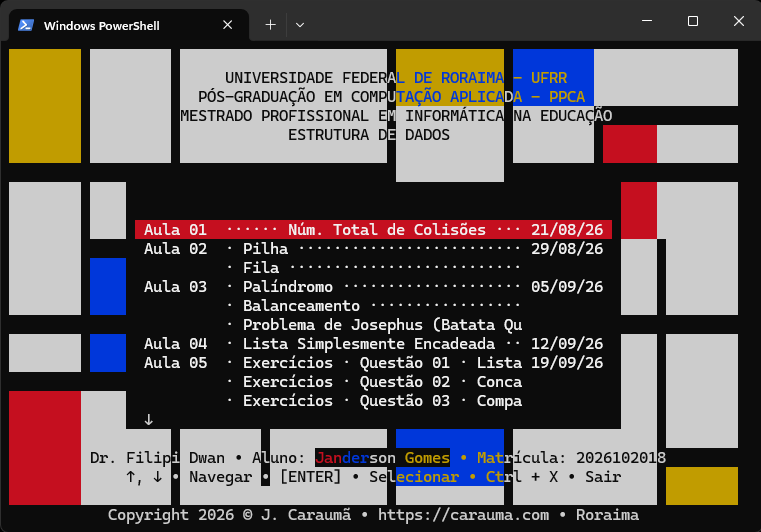
\includegraphics[width=0.60\linewidth]{img/repo_menu.png}
    \caption{Aplicação desenvolvida em C como trabalho final.}
    \label{fig:placeholder}
 \end{figure}
\end{frame}

\begin{frame}[fragile]{Quick Sort implementado (\texttt{quick-sort.c})}
\begin{lstlisting}[style=code]
static void quick_range(int *values, size_t left, size_t right,
                        Lesson11Metrics *metrics)
{
    size_t store = left, i;
    int pivot;
    if (right - left < 2) return;          /* caso base */
    pivot = values[right - 1];             /* pivô = último elemento */
    for (i = left; i + 1 < right; i++) {
        metrics->comparisons++;
        if (values[i] < pivot) {           /* troca i <-> store */
            int t = values[i]; values[i] = values[store]; values[store] = t;
            metrics->movements += 3;
            store++;
        }
    }
    /* troca values[store] <-> pivô (+3 movimentações) */
    quick_range(values, left, store, metrics);
    quick_range(values, store + 1, right, metrics);
}
\end{lstlisting}
 {\scriptsize Trecho adaptado (contadores de progresso omitidos): é a partição de Lomuto, em intervalo semiaberto $[left,right)$.}
\end{frame}

\begin{frame}{Tempos medidos (uma execução por tamanho)}
 \centering\scriptsize
 \renewcommand{\arraystretch}{1.3}
 \begin{tabular}{@{}lrrrr@{}}
  \toprule
  \textbf{Algoritmo} & $n=100$ & $n=1.000$ & $n=10.000$ & $n=100.000$\\
  \midrule
  \textcolor{mred}{\rule{0.9ex}{0.9ex}}\ \textbf{Quick Sort} & \textbf{6 µs} & \textbf{63 µs} & \textbf{701 µs} & \textbf{8 ms}\\
  Merge Sort & 9 µs & 89 µs & 911 µs & 10 ms\\
  Heap Sort & 6 µs & 83 µs & 1 ms & 11 ms\\
  Radix Sort & 14 µs & 108 µs & 911 µs & 9 ms\\
  Insertion Sort & 8 µs & 730 µs & 47 ms & 5 s\\
  Selection Sort & 15 µs & 1 ms & 74 ms & 7 s\\
  Bubble Sort & 22 µs & 2 ms & 117 ms & 15 s\\
  \bottomrule
 \end{tabular}
 \par\vspace{0.6em}
 {\scriptsize Fonte: Autor (2026).}
\end{frame}

\begin{frame}{Curvas obtidas $\times$ referências teóricas}
 \centering
 \begin{tikzpicture}
  \begin{axis}[mond,width=9.6cm,height=5.9cm,xmode=log,ymode=log,xlabel={$n$ (elementos)},ylabel={tempo ($\mu$s)},
   xmin=80,xmax=120000,ymin=3,ymax=30000000,xtick={100,1000,10000,100000},legend pos=outer north east,
    legend cell align=left]
  \addplot[mred,very thick,mark=square*,mark size=2pt] coordinates {(100,6)(1000,63)(10000,701)(100000,8000)}; \addlegendentry{Quick}
  \addplot[mblue,mark=triangle*,mark size=2pt] coordinates {(100,9)(1000,89)(10000,911)(100000,10000)}; \addlegendentry{Merge}
  \addplot[mblue,dashed,mark=diamond*,mark size=2pt] coordinates {(100,6)(1000,83)(10000,1000)(100000,11000)}; \addlegendentry{Heap}
  \addplot[mgold,mark=*,mark size=2pt] coordinates {(100,14)(1000,108)(10000,911)(100000,9000)}; \addlegendentry{Radix}
  \addplot[mink,mark=o,mark size=2pt] coordinates {(100,8)(1000,730)(10000,47000)(100000,5000000)}; \addlegendentry{Insertion}
  \addplot[mink,dashed,mark=x,mark size=2.4pt] coordinates {(100,15)(1000,1000)(10000,74000)(100000,7000000)}; \addlegendentry{Selection}
  \addplot[mink,dotted,mark=+,mark size=2.4pt] coordinates {(100,22)(1000,2000)(10000,117000)(100000,15000000)}; \addlegendentry{Bubble}
  \addplot[mred,thin,dashed,domain=2:5,samples=10]({10^x},{10^x*x*0.03}); \addlegendentry{ref. $n\log n$}
  \addplot[mink,thin,dashed,domain=2:5,samples=10]({10^x},{10^(2*x)*0.0008}); \addlegendentry{ref. $n^2$}
  \end{axis}
 \end{tikzpicture}
 \par\vspace{0.2em}
 {\scriptsize Referências tracejadas ancoradas no ponto $n=100$ (Quick: 6 µs; Insertion: 8 µs).}
\end{frame}

\begin{frame}{Crescimento observado $\times$ previsto}
 \centering\footnotesize
 \renewcommand{\arraystretch}{1.3}
 \begin{tabular}{@{}lccccccc@{}}
  \toprule
  & \multicolumn{2}{c}{\textbf{$100\to1.000$ (×)}} & \multicolumn{2}{c}{\textbf{$1.000\to10.000$ (×)}} & \multicolumn{2}{c}{\textbf{$10.000\to100.000$ (×)}} \\
  \cmidrule(lr){2-3}\cmidrule(lr){4-5}\cmidrule(lr){6-7}
  \textbf{Algoritmo} & observado & previsto & observado & previsto & observado & previsto & \textbf{Modelo}\\
  \midrule
  \textbf{Quick} & 10,5 & 15,0 & 11,1 & 13,3 & 11,4 & 12,5 & $n\log n$\\
  Merge & 9,9 & 15,0 & 10,2 & 13,3 & 11,0 & 12,5 & $n\log n$\\
  Heap & 13,8 & 15,0 & 12,0 & 13,3 & 11,0 & 12,5 & $n\log n$\\
  Radix & 7,7 & 10 & 8,4 & 10 & 9,9 & 10 & $d\,(n+b)$\\
  Insertion & 91 & 100 & 64 & 100 & 106 & 100 & $n^2$\\
  Selection & $\approx$67 & 100 & 74 & 100 & $\approx$95 & 100 & $n^2$\\
  Bubble & $\approx$91 & 100 & $\approx$59 & 100 & $\approx$128 & 100 & $n^2$\\
  \bottomrule
 \end{tabular}
 \par\vspace{0.7em}
 {\scriptsize %Previsto: $n\log_2 n$ cresce 15,0$\times$, 13,3$\times$ e 12,5$\times$; $n^2$ cresce 100$\times$. Valores com ``$\approx$'' dependem de tempos arredondados. 
 O Quick Sort acompanha $n\log n$ \cite{clrs22}.}
\end{frame}

\begin{frame}{Comparações realizadas}
 \centering\footnotesize
 \renewcommand{\arraystretch}{1.3}
 \begin{tabular}{@{}lrrrr@{}}
  \toprule
  \textbf{Algoritmo} & $n=100$ & $n=1.000$ & $n=10.000$ & $n=100.000$\\
  \midrule
  \textbf{Quick Sort} & \textbf{707} & \textbf{9.967} & \textbf{177.075} & \textbf{1.971.762}\\
  Merge Sort & 536 & 8.696 & 120.430 & 1.536.560\\
  Heap Sort & 1.042 & 16.844 & 235.352 & 3.019.814\\
  Insertion Sort & 2.554 & 252.542 & 24.960.251 & \textit{não medido}\\
  Selection Sort & 4.950 & 499.500 & 49.995.000 & 4.999.950.000\\
  Bubble Sort & 4.935 & 499.380 & 49.981.470 & \textit{não medido}\\
  Radix Sort & \multicolumn{4}{c}{sem comparações entre chaves (distribuição por dígitos)}\\
  \bottomrule
 \end{tabular}
 \par\vspace{0.6em}
 {\scriptsize Contagens recalculadas sobre os arquivos atuais \texttt{inteiros\_*.txt}; Insertion e Bubble em $n=100.000$ foram omitidos por serem quadráticos e levarem vários segundos.}
\end{frame}

\begin{frame}{Quick Sort: contagem observada $\times$ teoria}
 \begin{columns}[T]
  \column{0.35\textwidth}
   \centering
   \begin{tikzpicture}
    \begin{axis}[mond,width=6.6cm,height=5.3cm,xmode=log,ymode=log,xlabel={$n$},ylabel={comparações},
      xmin=80,xmax=120000,ymin=300,ymax=1e10,xtick={100,1000,10000,100000},legend pos=north west]
     \addplot[mink,dashed,mark=*,mark size=1.8pt] coordinates {(100,4950)(1000,499500)(10000,49995000)(100000,4999950000)}; \addlegendentry{pior $\frac{n(n-1)}{2}$}
     \addplot[mblue,mark=triangle*,mark size=2.2pt] coordinates {(100,648)(1000,10986)(10000,155772)(100000,2018053)}; \addlegendentry{média $2(n{+}1)H_n{-}4n$}
     \addplot[mred,very thick,mark=square*,mark size=2.2pt] coordinates {(100,707)(1000,9967)(10000,177075)(100000,1971762)}; \addlegendentry{observado (arquivos)}
    \end{axis}
   \end{tikzpicture}
  \column{0.41\textwidth}
   \footnotesize
   \begin{tabular}{@{}rrrr@{}}
    \toprule
    $n$ & obs. & teoria & desvio\\
    \midrule
    100 & 707 & 648 & $+9\%$\\
    1.000 & 9.967 & 10.986 & $-9\%$\\
    10.000 & 177.075 & 155.772 & $+14\%$\\
    100.000 & 1.971.762 & 2.018.053 & $-2\%$\\
    \bottomrule
   \end{tabular}
   \vspace{0.6em}\par
   \scriptsize
   \textbf{Validação:} 2.000 permutações aleatórias do mesmo algoritmo dão médias 647; 10.990; 155.825 (desvio-padrão 59; 639; 6.525), em acordo com a fórmula. O arquivo de $n=10.000$ fica $\approx3{,}4\sigma$ acima da média.\\[0.5ex]
   \textbf{Hipótese} (não testada): os bits baixos de um congruencial com módulo $2^{32}$ têm período curto \cite{knuth97}, e o valor é $x \bmod 10^5$; usar bits altos ou outro gerador deve aproximar o resultado da média.
 \end{columns}
\end{frame}

%\begin{frame}{Pior caso medido: entrada já ordenada}
% \begin{columns}[T]
%  \column{0.5\textwidth}
%   \centering\footnotesize
%   \renewcommand{\arraystretch}{1.3}
%   \begin{tabular}{@{}lrr@{}}
%    \toprule
%    \textbf{Entrada ($n{=}10^4$)} & \textbf{Comp.} & \textbf{Prof.}\\
%    \midrule
%    Aleatória (arquivo) & 177.708 & 36\\
%    Já ordenada & 49.995.000 & 9.999\\
%    \bottomrule
%   \end{tabular}
%   \par\vspace{0.6em}
%   {\scriptsize Prof. = profundidade máxima da recursão. Experimento adicional: mesmo código (pivô = último) sobre $0,1,\dots,9999$; não consta em \texttt{data/}.}
%  \column{0.46\textwidth}
%   \begin{alertblock}{Leitura}
%    \footnotesize
%    Com pivô fixo nas pontas, a entrada ordenada produz partições de tamanho $n-1$ e $0$: exatamente $\frac{n(n-1)}{2}=49.995.000$ comparações, o mesmo número do Selection Sort.\\[0.5ex]
%    A recursão chega a $\approx n$ níveis: em C, risco de \emph{estouro de pilha} para $n$ grande. Mitigações: pivô aleatório ou mediana de três, e recursão na menor parte.
%   \end{alertblock}
% \end{columns}
%\end{frame}

%\begin{frame}{Ordenar compensa? Ordenação $+$ busca binária}
% \begin{columns}[T]
%  \column{0.5\textwidth}
%   \footnotesize
%   Cenário do módulo de busca: vetor de $n=10.000$ e $q=10.000$ consultas aleatórias em $[0,\,99.999]$ (cerca de 90\% ausentes).
%   \vspace{0.6em}
%   \renewcommand{\arraystretch}{1.3}
%   \begin{tabular}{@{}p{3.6cm}r@{}}
%    \toprule
%    \textbf{Estratégia} & \textbf{Comp.}\\
%    \midrule
%    Sequencial (desordenado) & $\approx 9{,}5\times10^{7}$\\
%    Quick Sort + binária & $\approx 1{,}8\times10^{5}+1{,}3\times10^{5}$\\
%    \bottomrule
%   \end{tabular}
%  \column{0.42\textwidth}
%   \footnotesize
%   \begin{exampleblock}{Ponto de equilíbrio}
%    A ordenação (177.708 comparações medidas) se paga a partir de cerca de \textbf{18 buscas} com chave ausente: $q\,n \gtrsim C_{\text{sort}}+q\log_2 n$.
%   \end{exampleblock}
%   {\tiny Estimativa teórica: busca sequencial $\approx n$ comparações se ausente e $n/2$ se presente; busca binária $\approx\log_2 n\approx13$. Os tempos da busca em lote são medidos pelo módulo \texttt{search-benchmark.c}; seus resultados não estão salvos em \texttt{data/}.}
% \end{columns}
%\end{frame}

% Comparações
\setsec{mred}{mblue}
\secslide{7}{Comparações com\\outros algoritmos}{mred}{mblue}{myel}{white}

\begin{frame}{Tabela comparativa (teoria)}
 \centering\scriptsize
 \renewcommand{\arraystretch}{1.3}
 \begin{tabular}{@{}lccclcc@{}}
  \toprule
  \textbf{Algoritmo} & \textbf{Melhor} & \textbf{Médio} & \textbf{Pior} & \textbf{Memória extra} & \textbf{Estável} & \textbf{In-place}\\
  \midrule
  Selection & $n^2$ & $n^2$ & $n^2$ & $O(1)$ & não & sim\\
  Insertion & $n$ & $n^2$ & $n^2$ & $O(1)$ & sim & sim\\
  Bubble (com parada) & $n$ & $n^2$ & $n^2$ & $O(1)$ & sim & sim\\
  Radix (LSD) & $d(n{+}b)$ & $d(n{+}b)$ & $d(n{+}b)$ & $O(n{+}b)$ & sim & não\\
  \textcolor{mred}{\rule{0.8ex}{0.8ex}}\ \textbf{Quick} & $n\log n$ & $n\log n$ & $n^2$ & $O(\log n)$ esp.; $O(n)$ pior & não & sim\\
  Merge & $n\log n$ & $n\log n$ & $n\log n$ & $O(n)$ & sim & não\\
  Heap & $n\log n$ & $n\log n$ & $n\log n$ & $O(1)$ & não & sim\\
  \bottomrule
 \end{tabular}
 \par\vspace{0.6em}
 {\scriptsize Notação: $\Theta(\cdot)$ para tempo; $d$ = dígitos, $b$ = base. Valores conforme \cite{clrs22,knuth98,ziviani10} e as anotações do próprio repositório.}
\end{frame}

\begin{frame}{Quick $\times$ Merge $\times$ Heap: quando preferir cada um}
 \centering\footnotesize
 \renewcommand{\arraystretch}{1.35}
 \begin{tabular}{@{}p{2.5cm}p{2.9cm}p{2.9cm}p{2.9cm}@{}}
  \toprule
  & \textbf{Quick Sort} & \textbf{Merge Sort} & \textbf{Heap Sort}\\
  \midrule
  Pior caso & $\Theta(n^2)$ (evitável) & $\Theta(n\log n)$ & $\Theta(n\log n)$\\
  Memória extra & pilha $O(\log n)$ & vetor auxiliar $O(n)$ & $O(1)$\\
  Estabilidade & não & sim & não\\
  Acesso à memória & sequencial; boa localidade de cache & sequencial; exige cópias & saltos pela árvore; má localidade\\
  Comparações (medido, $n=10^5$) & 1.971.762 & 1.536.560 & 3.019.814\\
  Tempo (medido, $n=10^5$) & 8 ms & 10 ms & 11 ms\\
  Indicado para & vetores em memória, uso geral & estabilidade; listas; dados externos & memória mínima e garantia de pior caso\\
  \bottomrule
 \end{tabular}
 \par\vspace{0.4em}
 {\scriptsize O Merge Sort faz menos comparações, mas o Quick Sort compensa com menor custo por operação (sem cópias para vetor auxiliar), resultando em tempos equivalentes na escala medida \cite{sedgewick11}.}
\end{frame}

% Usos, vantagens, limitações
\setsec{mblue}{mred}
\secslide{8}{Usos, vantagens, limitações}{mblue}{myel}{mred}{white}

\begin{frame}{Vantagens e desvantagens}
 \begin{columns}[T]
  \column{0.4\textwidth}
   \begin{block}{Vantagens}
    \footnotesize
    \begin{itemize}
     \item Em média $\Theta(n\log n)$, com constante pequena (cerca de $1{,}39\,n\log_2 n$ comparações).
     \item \emph{In-place}: sem vetor auxiliar; apenas pilha $O(\log n)$.
     \item Boa localidade de referência (varredura sequencial).
     \item Pouco código; fácil de adaptar (3 vias, \emph{quickselect}, paralelismo).
     \item Base de implementações de bibliotecas \cite{bentleymcilroy93,musser97}.
    \end{itemize}
   \end{block}
  \column{0.4\textwidth}
   \begin{alertblock}{Desvantagens}
    \footnotesize
    \begin{itemize}
     \item Pior caso $\Theta(n^2)$ com pivôs ruins; entradas adversárias existem \cite{mcilroy99}.
     \item Não é estável.
     \item Recursão profunda no pior caso (risco de estouro de pilha).
     \item Sensível a muitos valores repetidos se a partição for de duas vias.
     \item Desempenho depende da escolha do pivô e de detalhes de implementação.
    \end{itemize}
   \end{alertblock}
 \end{columns}
\end{frame}

\begin{frame}{Por que usar o Quick Sort?}
 \begin{enumerate}
  \item \textbf{Ordenação geral em memória:} é a escolha padrão quando não se exige estabilidade e se quer pouca memória extra.
  \item \textbf{Desempenho prático:} constantes baixas e cache amigável; nos experimentos, o menor tempo em todos os tamanhos medidos (6 µs, 63 µs, 701 µs e 8 ms).
  \item \textbf{Robustez com engenharia:} pivô aleatório/mediana de três, corte para inserção e Introsort eliminam o pior caso na prática \cite{sedgewick78,musser97}.
  \item \textbf{Ideia reutilizável:} a mesma partição resolve seleção do $k$-ésimo elemento (\emph{quickselect}) \cite{hoare61find,clrs22}.
 \end{enumerate}
 \vspace{0.6em}
 \begin{alertblock}{Quando evitar}
  \footnotesize Quando é preciso \textbf{estabilidade} (usar Merge/Timsort), \textbf{pior caso garantido} sem engenharia adicional (Heap/Merge/Introsort) ou dados em \textbf{memória externa} (intercalação).
 \end{alertblock}
\end{frame}

\begin{frame}{Principais usos na literatura}
 \centering\footnotesize
 \renewcommand{\arraystretch}{1.3}
 \begin{tabular}{@{}p{2.8cm}p{4.8cm}p{3.4cm}@{}}
  \toprule
  \textbf{Contexto} & \textbf{Uso} & \textbf{Fonte}\\
  \midrule
  C++ & \texttt{std::sort} é tipicamente um Introsort (Quick Sort + Heap Sort + inserção) & \cite{musser97}\\
  Java & \texttt{Arrays.sort} para tipos primitivos usa Dual-Pivot Quicksort & \cite{wildnebel12}\\
  Go & pacote \texttt{sort} usa pdqsort desde a versão 1.19 & \cite{peters21}\\
  Seleção & mediana e $k$-ésimo menor em tempo esperado $O(n)$ (\emph{quickselect}) & \cite{hoare61find,clrs22}\\
  Competições (ICPC, OBI, Maratona SBC) & usa-se o \texttt{sort} da biblioteca; adversários clássicos contra Quick Sort ingênuo motivam pivô aleatório e Introsort & \cite{mcilroy99}\\
  Ensino & Knuth (\S5.2.2), Cormen et al.\ (cap.\ 7), Sedgewick e Wayne (\S2.3) & \cite{knuth98,clrs22,sedgewick11}\\
  \bottomrule
 \end{tabular}
\end{frame}

\begin{frame}{Onde estudar mais?}
 \begin{columns}[T]
  \column{0.4\textwidth}
   \footnotesize
   \textbf{Internacionais}
   \begin{itemize}
    \item \textbf{D. E. Knuth}, \emph{The Art of Computer Programming}, vol.\ 3: análise detalhada do Quick Sort em \S5.2.2 \cite{knuth98}.
    \item \textbf{Cormen, Leiserson, Rivest e Stein}: capítulo 7, partições de Lomuto e Hoare, análise e aleatorização \cite{clrs22}.
    \item \textbf{R. Sedgewick}: otimizações práticas \cite{sedgewick78} e \emph{Algorithms}, \S2.3 \cite{sedgewick11}.
    \item \textbf{J. Bentley}: \emph{Programming Pearls} \cite{bentley00}.
   \end{itemize}
  \column{0.4\textwidth}
   \footnotesize
   \textbf{Em português}
   \begin{itemize}
    \item \textbf{N. Ziviani}, \emph{Projeto de Algoritmos com Implementações em Pascal e C} \cite{ziviani10}.
    \item \textbf{Celes, Cerqueira e Rangel}, \emph{Introdução a Estruturas de Dados com Técnicas de Programação em C} \cite{celes17}.
    \item \textbf{Szwarcfiter e Markenzon}, \emph{Estruturas de Dados e seus Algoritmos} \cite{szwarcfiter10}.
    \item \textbf{P. Feofiloff}, \emph{Algoritmos em Linguagem C} \cite{feofiloff09}.
   \end{itemize}
 \end{columns}
\end{frame}

%\begin{frame}{Conclusões}
% \begin{itemize}
%  \item O Quick Sort nasce de uma ideia simples (partição + recursão) e, desde 1961, continua como base dos principais \emph{sorts} de biblioteca.
%  \item \textbf{Teoria:} $\Theta(n\log n)$ em média, $\Theta(n^2)$ no pior caso; \textbf{prática:} o pior caso é evitado por pivô aleatório, mediana de três e Introsort.
%  \item \textbf{Nos experimentos do repositório:} menor tempo entre os sete algoritmos em $n=100$, $1.000$ e $10.000$; crescimento coerente com $n\log n$; contagem de comparações próxima da fórmula (+14\% em $n=10.000$, com hipótese de gerador discutida).
%  \item \textbf{Limitações:} uma execução por tamanho, tempos arredondados no nome do arquivo, $n\le10^4$ e um único tipo de entrada.
% \end{itemize}
% \vspace{0.4em}
% \begin{exampleblock}{Trabalhos futuros}
%  \footnotesize Repetir as medições (mediana de 30 execuções), incluir $n=10^5$ e $10^6$, entradas ordenadas/inversas/com repetições, comparar Lomuto $\times$ Hoare $\times$ três vias $\times$ mediana de três $\times$ Introsort e adotar um gerador pseudoaleatório de melhor qualidade.
% \end{exampleblock}
%\end{frame}

% Conclusão
\begin{frame}[plain]
 \begin{tikzpicture}[remember picture,overlay]
  \begin{scope}[shift={(current page.south west)}]
   \fill[mpaper] (0,0) rectangle (16,9);
   \fill[mblue] (0,0) rectangle (3.0,4.2);
   \fill[mred] (13.14,6.64) rectangle (16,9);
   \fill[myel] (13.14,0) rectangle (16,1.86);
   \fill[mink] (3.0,0) rectangle (3.14,9);
   \fill[mink] (13.0,0) rectangle (13.14,9);
   \fill[mink] (0,4.2) rectangle (16,4.34);
   \fill[mink] (3.14,1.72) rectangle (16,1.86);
   \fill[mink] (3.14,6.5) rectangle (16,6.64);
   \node[anchor=west,font=\fontsize{40}{44}\bfseries] at (3.6,5.5) {Obrigado!};
   \node[anchor=west,font=\large,text width=8.8cm] at (3.6,3.2) {Viva o software livre!};
   \node[anchor=west,font=\small,text=mgrey,text width=8.8cm] at (3.6,2.55)
     {\copyright \ Caraumã (\href{https://carauma.com}{carauma.com}) \,·\, Orgulhosamente feito em \LaTeX};
   %\node[anchor=west,font=\large,text width=8.8cm] at (3.6,3.2) {Perguntas e discussão};
   %\node[anchor=west,font=\small,text=mgrey,text width=8.8cm] at (3.6,2.55)
   %  {\autor\ \,·\, \url{https://github.com/carauma7/art-mondrian}};
   \node[anchor=center, inner sep=0pt] at (1.37, 6.8) {
       
\includegraphics[width=2.5cm]{img/carauma.png}
   };
  \end{scope}
 \end{tikzpicture}
\end{frame}

% Referências
\setsec{mred}{myel}
\begin{frame}[allowframebreaks]{Referências}
 \begin{thebibliography}{99}
  \bibitem[Bentley, 2000]{bentley00} J. Bentley. \emph{Programming Pearls}. 2.\,ed. Addison-Wesley, 2000.
  \bibitem[Bentley e McIlroy, 1993]{bentleymcilroy93} J. L. Bentley, M. D. McIlroy. Engineering a sort function. \emph{Software: Practice and Experience}, 23(11):1249--1265, 1993.
  \bibitem[Celes et al., 2017]{celes17} W. Celes, R. Cerqueira, J. L. Rangel. \emph{Introdução a Estruturas de Dados com Técnicas de Programação em C}. 2.\,ed. Elsevier, 2016.
  \bibitem[Cormen et al., 2022]{clrs22} T. H. Cormen, C. E. Leiserson, R. L. Rivest, C. Stein. \emph{Introduction to Algorithms}. 4.\,ed. MIT Press, 2022. (cap.\,7, Quicksort)
  \bibitem[Dijkstra, 1976]{dijkstra76} E. W. Dijkstra. \emph{A Discipline of Programming}. Prentice-Hall, 1976.
  \bibitem[Edelkamp e Weiss, 2016]{edelkampweiss16} S. Edelkamp, A. Weiss. BlockQuicksort: how branch mispredictions don't affect quicksort. In: \emph{ESA 2016}, LIPIcs 57, 38:1--38:16, 2016.
  \bibitem[Feofiloff, 2009]{feofiloff09} P. Feofiloff. \emph{Algoritmos em Linguagem C}. Elsevier/Campus, 2009.
  \bibitem[Hoare, 1961a]{hoare61} C. A. R. Hoare. Algorithm 64: Quicksort. \emph{Communications of the ACM}, 4(7):321, 1961.
  \bibitem[Hoare, 1961b]{hoare61find} C. A. R. Hoare. Algorithm 65: Find. \emph{Communications of the ACM}, 4(7):321--322, 1961.
  \bibitem[Hoare, 1962]{hoare62} C. A. R. Hoare. Quicksort. \emph{The Computer Journal}, 5(1):10--16, 1962.
  \bibitem[Knuth, 1997]{knuth97} D. E. Knuth. \emph{The Art of Computer Programming}, vol.\,2: Seminumerical Algorithms. 3.\,ed. Addison-Wesley, 1997. (cap.\,3, números aleatórios)
  \bibitem[Knuth, 1998]{knuth98} D. E. Knuth. \emph{The Art of Computer Programming}, vol.\,3: Sorting and Searching. 2.\,ed. Addison-Wesley, 1998. (\S5.2.2)
  \bibitem[McIlroy, 1999]{mcilroy99} M. D. McIlroy. A killer adversary for quicksort. \emph{Software: Practice and Experience}, 29(4):341--344, 1999.
  \bibitem[Musser, 1997]{musser97} D. R. Musser. Introspective sorting and selection algorithms. \emph{Software: Practice and Experience}, 27(8):983--993, 1997.
  \bibitem[Peters, 2021]{peters21} O. R. L. Peters. Pattern-defeating quicksort. \emph{arXiv}:2106.05123, 2021.
  \bibitem[Sedgewick, 1978]{sedgewick78} R. Sedgewick. Implementing Quicksort programs. \emph{Communications of the ACM}, 21(10):847--857, 1978.
  \bibitem[Sedgewick e Wayne, 2011]{sedgewick11} R. Sedgewick, K. Wayne. \emph{Algorithms}. 4.\,ed. Addison-Wesley, 2011. (\S2.3)
  \bibitem[Shustek, 2009]{shustek09} L. Shustek. An interview with C.A.R. Hoare. \emph{Communications of the ACM}, 52(3):38--41, 2009.
  \bibitem[Szwarcfiter e Markenzon, 2010]{szwarcfiter10} J. L. Szwarcfiter, L. Markenzon. \emph{Estruturas de Dados e seus Algoritmos}. 3.\,ed. LTC, 2010.
  \bibitem[Wild e Nebel, 2012]{wildnebel12} S. Wild, M. E. Nebel. Average case analysis of Java 7's dual pivot quicksort. In: \emph{ESA 2012}, LNCS 7501, p.\,825--836, Springer, 2012.
  \bibitem[Ziviani, 2010]{ziviani10} N. Ziviani. \emph{Projeto de Algoritmos com Implementações em Pascal e C}. 3.\,ed. Cengage Learning, 2010.
 \end{thebibliography}
\end{frame}

% Apêndice (Código pra demonstração)
\begin{frame}[fragile]{Apêndice: programa de demonstração em C}
 \begin{columns}[T]
  \column{0.5\textwidth}
\begin{lstlisting}[style=code]
#include <stdio.h>
static void troca(int *a, int *b) {
    int t = *a; *a = *b; *b = t;
}
static int particionar(int A[],
                       int lo, int hi) {
    int pivo = A[hi], s = lo;     /* Lomuto */
    for (int i = lo; i < hi; i++)
        if (A[i] < pivo)
            troca(&A[i], &A[s++]);
    troca(&A[s], &A[hi]);
    return s;
}
void quicksort(int A[], int lo, int hi) {
    if (lo < hi) {
        int p = particionar(A, lo, hi);
        quicksort(A, lo, p - 1);
        quicksort(A, p + 1, hi);
    }
}
\end{lstlisting}
  \column{0.4\textwidth}
\begin{lstlisting}[style=code]
int main(void) {
    int A[] = {7, 2, 9, 4, 6, 5};
    quicksort(A, 0, 5);
    for (int i = 0; i < 6; i++)
        printf("%d ", A[i]);
    printf("\n"); /* 2 4 5 6 7 9 */
    return 0;
}
\end{lstlisting}
   \vspace{0.6em}
   {\scriptsize Compilar:\\ \texttt{gcc -Wall -O2 quicksort.c}\\ \texttt{\ \ -o quicksort}\\[0.8ex]
   As variantes de Hoare, três vias e mediana de três usam a mesma função \texttt{troca}.}
 \end{columns}
\end{frame}


\end{document}